\documentclass[12pt,titlepage]{article}
\usepackage[margin=1.25in]{geometry}
\usepackage{graphicx,amsmath,blindtext,minted}

%% Variables definition
\newcommand{\vSubject}{Data Structure and Algorithm Practicum}
\newcommand{\vSubtitle}{Double Linked Lists}
\newcommand{\vName}{Muhammad Baihaqi Aulia Asy'ari}
\newcommand{\vNIM}{2241720145}
\newcommand{\vClass}{1I}
\newcommand{\vDepartment}{Information Technology}
\newcommand{\vStudyProgram}{D4 Informatics Engineering}

%% [START] Tikz related stuff
\usepackage{tikz}
\usetikzlibrary{svg.path,calc,shapes.geometric,shapes.misc}
\tikzstyle{terminator} = [rectangle, draw, text centered, rounded corners = 1em, minimum height=2em]
\tikzstyle{preparation} = [chamfered rectangle, chamfered rectangle sep=0.75em, draw, text centered, minimum height = 2em]
\tikzstyle{process} = [rectangle, draw, text centered, minimum height=2em]
\tikzstyle{decision} = [diamond, aspect=2, draw, text centered, minimum height=2em]
\tikzstyle{data}=[trapezium, draw, text centered, trapezium left angle=60, trapezium right angle=120, minimum height=2em]
\tikzstyle{connector} = [line width=0.25mm,->]
%% [END] Tikz related stuff

%% [START] Fancy header related stuff
\usepackage{fancyhdr}
\pagestyle{fancy}
\setlength{\headheight}{15pt} % compensate fancyhdr style
\fancyhead{}
\fancyfoot{}
\fancyfoot[L]{\thepage}
\fancyfoot[R]{\textit{\vSubject - \vSubtitle}}
\renewcommand{\footrulewidth}{0.4pt}% default is 0pt, overline for footer
%% [END] Fancy header related stuff

%% [START] Custom tabular command related stuff
\usepackage{tabularx}
\newcommand{\details}[2]{
    #1 & #2  \\
}
%% [END] Custom tabular command related stuff

%% [START] Figure related stuff
\newcommand{\image}[3][1]{
    \begin{figure}[h]
        \centering
        \includegraphics[#1]{#2}
        \caption{#3}
        \label{#3}
    \end{figure}
}
%% [END] Figure related stuff

%%
\usepackage{pgf-umlcd}

\renewcommand{\umldrawcolor}{black}
\renewcommand{\umlfillcolor}{white}
%%

%% [BEGIN] Custom enumerator
\usepackage{enumitem}
%% [END] Custom enumerator

%% [BEGIN] Paragraph indent
\usepackage{indentfirst}
%% [END] Paragraph indent

\begin{document}
\begin{titlepage}
    \centering
    \vfill
    {\bfseries\LARGE
        \vSubject\\
        \vskip0.25cm
        \vSubtitle
    }
    \vfill
    \includegraphics[width=6cm]{images/polinema-logo.png}
    \vfill
    {
        \textbf{Name}\\
        \vName\\
        \vskip0.5cm
        \textbf{NIM}\\
        \vNIM\\
        \vskip0.5cm
        \textbf{Class}\\
        \vClass\\
        \vskip0.5cm
        \textbf{Department}\\
        \vDepartment\\
        \vskip0.5cm
        \textbf{Study Program}\\
        \vStudyProgram
    }
\end{titlepage}

\newpage

\setcounter{section}{1}
\subsection{Learning Objective}
After learning this lab activity, students will be able to:
\begin{enumerate}
    \item Understand Double Linked List algorithm
    \item Create and declare double linked list algorithm
    \item Implement double linked list algorithm in various case studies
\end{enumerate}

\subsection{Lab Activities 1}
In this lab activity, we will create Node class and DoubleLinkedList class that has operations to insert data in multiple way. (from the beginning or the tail of the list)

\subsubsection{Steps}
\begin{enumerate}
    \item Take this class diagram as your reference for creating the \textbf{DoubleLinkedList class}
    \mbox{}\\
    \mbox{}\\
    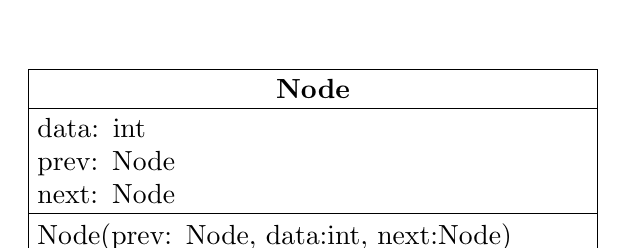
\begin{tikzpicture}
        \begin{class}[text width=7cm]{Node}{0,0}
            \attribute{data: int}
            \attribute{prev: Node}
            \attribute{next: Node}
            \operation{Node(prev: Node, data:int, next:Node)}
        \end{class}
    \end{tikzpicture}
    \mbox{}\\
    \mbox{}\\
    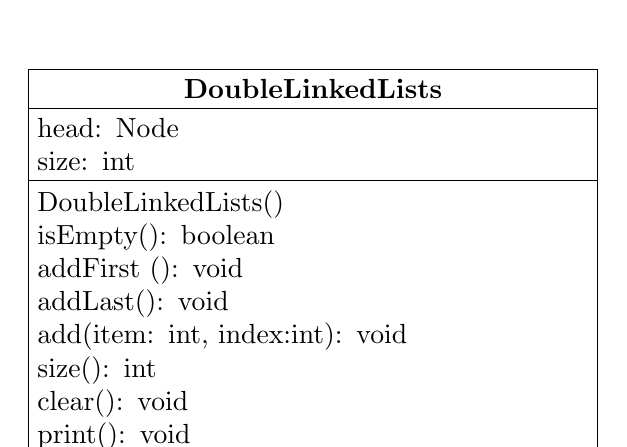
\begin{tikzpicture}
        \begin{class}[text width=7cm]{DoubleLinkedLists}{0,0}
            \attribute{head: Node}
            \attribute{size: int}
            \operation{DoubleLinkedLists()}
            \operation{isEmpty(): boolean}
            \operation{addFirst (): void}
            \operation{addLast(): void}
            \operation{add(item: int, index:int): void}
            \operation{size(): int}
            \operation{clear(): void}
            \operation{print(): void}
        \end{class}
    \end{tikzpicture}
    \mbox{}\\
    \item Create a new package named \textbf{DoubleLinkedList}
    \item Create a new class in that package named \textbf{Node}
    \item In that class, declare the attributes as described in the class diagram
    \begin{minted}[autogobble,breaklines]{java}
        int data;
        Node prev, next;
    \end{minted}
    \item Next, add the default constructor in Node class
    \begin{minted}[autogobble,breaklines]{java}
        public Node(Node prev, int data, Node next) {
            this.data = data;
            this.prev = prev;
            this.next = next;
        }
    \end{minted}
    \item Create a new class named \textbf{DoubleLinkedList} in the same package with the node as following image:
    \begin{minted}[autogobble,breaklines]{java}
        package LabActivities;

        public class DoubleLinkedList {
        
        }
    \end{minted}
    \item Next, we add the attributes
    \begin{minted}[autogobble,breaklines]{java}
        Node head;
        int size;
    \end{minted}
    \item Then, add the constructor in class \textbf{DoubleLinkedList}
    \begin{minted}[autogobble,breaklines]{java}
        public DoubleLinkedList() {
            head = null;
            size = 0;
        }
    \end{minted}
    \item Create method isEmpty(), this method will be used to check whether the linked list is empty or not
    \begin{minted}[autogobble,breaklines]{java}
        public boolean isEmpty() {
            return head == null;
        }
    \end{minted}
    \item Then add method \textbf{addFirst()}. This method will be executed when we want to add data in the beginning of the list
    \begin{minted}[autogobble,breaklines]{java}
        public void addFirst(int item) {
            if (isEmpty()) {
                head = new Node(null, item, null);
            } else {
                Node newNode = new Node(null, item, head);
                head.prev = newNode;
                head = newNode;
            }
            size++;
        }
    \end{minted}
    \item Let’s not forget about adding the data in the end of the list. We can do it after adding these lines of code in \textbf{addLast()} method
    \begin{minted}[autogobble,breaklines]{java}
        public void addLast(int item) {
            if (isEmpty()) {
                addFirst(item);
            } else {
                Node current = head;
                while (current.next != null) {
                    current = current.next;
                }
                Node newNode = new Node(current, item, null);
                current.next = newNode;
                size++;
            }
        }
    \end{minted}
    \item If we want to add a data that specified by a certain index, we will need to provide additional method to do so. It can be done by creating the \textbf{add()} method
    \begin{minted}[autogobble,breaklines]{java}
        public void add(int item, int index) throws Exception{
            if (isEmpty()) {
                addFirst(item);
            } else if (index < 0 || index > size) {
                throw new Exception("Index out of bound");
            } else {
                Node current = head;
                int i = 0;
                while (i < index) {
                    current = current.next;
                    i++;
                }
                if (current.next == null) {
                    Node newNode = new Node(null, item, current);
                    current.prev = newNode;
                    head = newNode;
                } else {
                    Node newNode = new Node(current.prev, item, current);
                    newNode.prev = current.prev;
                    newNode.next = current;
                    current.prev.next = newNode;
                    current.prev = newNode;
                }
            }
            size++;
        }
    \end{minted}
    \item We want to make our list has an easy access to retrieve the length of the list. That’s why we create method \textbf{size()}
    \begin{minted}[autogobble,breaklines]{java}
        public int size() {
            return size;
        }
    \end{minted}
    \item We create a method \textbf{clear()} to remove all the data that are exist in linked lists
    \begin{minted}[autogobble,breaklines]{java}
        public void clear() {
            head = null;
            size = 0;
        }
    \end{minted}
    \item Next up, to print the whole data in the list, we need to create a method print().
    \begin{minted}[autogobble,breaklines]{java}
        public void print() {
            if (!isEmpty()) {
                Node temp = head;
                while (temp != null) {
                    System.out.print(temp.data + "\t");
                    temp = temp.next;
                }
                System.out.println("\n successfully added");
            } else {
                System.out.println("Linked list is empty");
            }
        }
    \end{minted}
    \item After creating the blueprint classes, we will need one main class so that all of that can be included in the program. Create \textbf{DoubleLinkedListMain} class to do so
    \begin{minted}[autogobble,breaklines]{java}
        package LabActivities;

        public class DoubleLinkedListMain {
            public static void main(String[] args) throws Exception {

            }
        }
    \end{minted}
    \item Instantiate an object from \textbf{DoubleLinkedList} class in the main method. Then apply these program code
    \begin{minted}[autogobble,breaklines]{java}
        DoubleLinkedList dll = new DoubleLinkedList();
        dll.print();
        System.out.println("Size: " + dll.size);
        System.out.println("================================================");
        dll.addFirst(3);
        dll.addLast(4);
        dll.addFirst(7);
        dll.print();
        System.out.println("Size: " + dll.size);
        System.out.println("================================================");
        dll.add(40, 1);
        dll.print();
        System.out.println("Size: " + dll.size);
        System.out.println("================================================");
        dll.clear();
        dll.print();
        System.out.println("Size: " + dll.size);
    \end{minted}
\end{enumerate}

\subsubsection{Result}
Compile the program and see if the result matches with following image
\begin{minted}[autogobble,breaklines,linenos]{text}
    PS D:\Kuliah\Smt 2\Algoritma dan Struktur Data\Praktikum\Week 12\Double Linked Lists>  d:; cd 'd:\Kuliah\Smt 2\Algoritma dan Struktur Data\Praktikum\Week 12\Double Linked Lists'; & 'C:\Program Files\Java\jdk-18.0.2.1\bin\java.exe' '-XX:+ShowCodeDetailsInExceptionMessages' '-cp' 'D:\Kuliah\Smt 2\Algoritma dan Struktur Data\Praktikum\Week 12\Double Linked Lists\bin' 'LabActivities.DoubleLinkedListMain'
    Linked list is empty
    Size: 0
    ================================================
    7       3       4
    successfully added
    Size: 3
    ================================================
    7       40      3       4
    successfully added
    Size: 4
    ================================================
    Linked list is empty
    Size: 0
\end{minted}

\subsubsection{Questions}
\begin{enumerate}
    \item What’s the difference between single linked list and double linked list?
    \mbox{}\\
    \texttt{Answer: }
    \mbox{}\\
    single linked list has tail and doesn't have prev in the node.
    \item In \textbf{Node class}, what is the usage of attribute next and prev ?
    \mbox{}\\
    \texttt{Answer: }
    \mbox{}\\
    to access prev and next node so that the node can go both way in the linked list.
    \item In constructor of \textbf{DoubleLinkedList} class. What’s the purpose of head and size attribute in this following code?
    \mbox{}\\
    \texttt{Answer: }
    \mbox{}\\
    head is use as a point of start of the linked list. and size is used to identify the linked list size to be able to insert data with index.
    \item In method \textbf{addFirst()}, why do we initialize the value of Node object to be null at first?
    \begin{minted}[autogobble,breaklines]{java}
        Node newNode = new Node(null, item, head);
    \end{minted}
    \mbox{}\\
    \texttt{Answer: }
    \mbox{}\\
    because the newNode will be placed at the head of the linked list. thus the Node prev is going to be null because it will be potition at head.
    \item In method \textbf{addLast()}, what’s the purpose of creating a node object by passing the \textbf{prev} parameter with \textbf{current} and \textbf{next} with \textbf{null} ?
    \begin{minted}[autogobble,breaklines]{java}
        Node newNode = new Node(current, item, null);
    \end{minted}
    \mbox{}\\
    \texttt{Answer: }
    \mbox{}\\
    because if the newNode is going to be placed at the last potition, the node current at the last potition is going to be need to be linked with the newNode prev Node. and because it is going to be placed in the last potition, the node next is going to be null.
\end{enumerate}

\subsection{Lab Activities 2}
In this lab activity, we have added some methods from our 1\textsuperscript{st} lab activity. Now, we added some ways for the users to remove a data in the beginning of the list, the tail, or with specified index. For more details, pay attention to this class diagram:
\mbox{}\\
\mbox{}\\
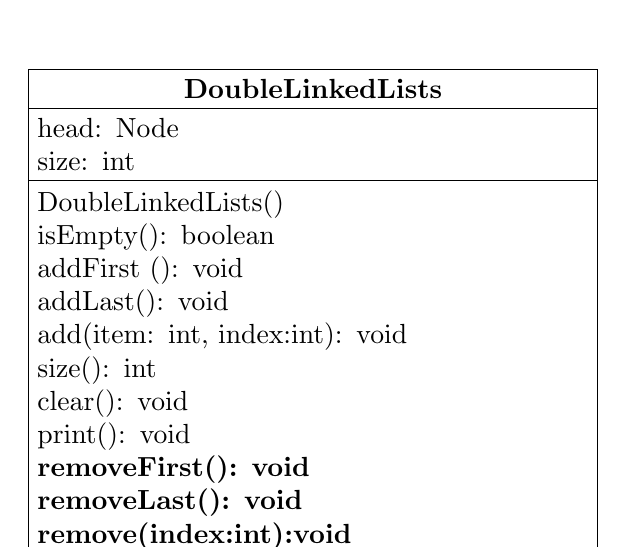
\begin{tikzpicture}
    \begin{class}[text width=7cm]{DoubleLinkedLists}{0,0}
        \attribute{head: Node}
        \attribute{size: int}
        \operation{DoubleLinkedLists()}
        \operation{isEmpty(): boolean}
        \operation{addFirst (): void}
        \operation{addLast(): void}
        \operation{add(item: int, index:int): void}
        \operation{size(): int}
        \operation{clear(): void}
        \operation{print(): void}
        \operation{ \textbf{removeFirst(): void}}
        \operation{ \textbf{removeLast(): void}}
        \operation{ \textbf{remove(index:int):void}}
    \end{class}
\end{tikzpicture}
\mbox{}\\

\subsubsection{Steps}
\begin{enumerate}
    \item Create method \textbf{removeFirst()} in class \textbf{DoubleLinkedList}
    \begin{minted}[autogobble,breaklines]{java}
        public void removeFirst() throws Exception{
            if (isEmpty()) {
                throw new Exception("Linked list is still empty, cannot remove data");
            } else if (size == 1) {
                removeLast();
            } else {
                head = head.next;
                head.prev = null;
                size--;
            }
        }
    \end{minted}
    \item Create method \textbf{removeLast()} in class \textbf{DoubleLinkedList}
    \begin{minted}[autogobble,breaklines]{java}
        public void removeLast() throws Exception{
            if (isEmpty()) {
                throw new Exception("Linked list is still empty, cannot remove data");
            } else if (head.next == null) {
                head = null;
                size--;
                return;
            } 
            Node current = head;
            while (current.next.next != null) {
                current = current.next;
            }
            current.next = null;
            size--;
        }
    \end{minted}
    \item Create method \textbf{remove()} in class \textbf{DoubleLinkedList}, alongside with its parameter
    \begin{minted}[autogobble,breaklines]{java}
        public void remove(int index) throws Exception{
            if (isEmpty() || index >= size) {
                throw new Exception("Index value is out of bound");
            } else if (size == 0) {
                removeFirst();
            } else {
                Node current = head;
                int i = 0;
                while (i < index) {
                    current = current.next;
                    i++;
                }
                if (current.next == null) {
                    current.prev.next = null;
                } else if (current.prev == null) {
                    current = current.next;
                    current.prev = null;
                    head = current;
                } else {
                    current.prev.next = current.next;
                    current.next.prev = current.prev;
                }
                size--;
            }
        }
    \end{minted}
    \item To execute additional codes we’ve just added, also make addition in the main class as well
    \begin{minted}[autogobble,breaklines]{java}
        dll.addLast(50);
        dll.addLast(40);
        dll.addLast(10);
        dll.addLast(20);
        dll.print();
        System.out.println("Size: " + dll.size);
        System.out.println("================================================");
        dll.removeFirst();
        dll.print();
        System.out.println("Size: " + dll.size);
        System.out.println("================================================");
        dll.removeLast();
        dll.print();
        System.out.println("Size: " + dll.size);
        System.out.println("================================================");
        dll.remove(1);
        dll.print();
        System.out.println("Size: " + dll.size);
    \end{minted}
\end{enumerate}

\subsubsection{Result}
Compile the program and see if the result matches with following image
\begin{minted}[autogobble,breaklines,linenos]{text}
    PS D:\Kuliah\Smt 2\Algoritma dan Struktur Data\Praktikum\Week 12\Double Linked Lists>  d:; cd 'd:\Kuliah\Smt 2\Algoritma dan Struktur Data\Praktikum\Week 12\Double Linked Lists'; & 'C:\Program Files\Java\jdk-18.0.2.1\bin\java.exe' '-XX:+ShowCodeDetailsInExceptionMessages' '-cp' 'D:\Kuliah\Smt 2\Algoritma dan Struktur Data\Praktikum\Week 12\Double Linked Lists\bin' 'LabActivities.DoubleLinkedListMain' 
    50      40      10      20
    successfully added
    Size: 4
    ================================================
    40      10      20
    successfully added
    Size: 3
    ================================================
    40      10
    successfully added
    Size: 2
    ================================================
    40
    successfully added
    Size: 1
\end{minted}

\subsubsection{Questions}
\begin{enumerate}
    \item What’s the meaning of these statements in \textbf{removeFirst()} method?
    \mbox{}\\
    \texttt{Answer: }
    \mbox{}\\
    it remove node it the head potition.
    \item How do we detect the position of the data that are in the last index in method \textbf{removeLast()}?
    \mbox{}\\
    \texttt{Answer: }
    \mbox{}\\
    loop through the linked list until the node next is null.
    \item Explain why this program code is not suitable if we include it in \textbf{remove} command!
    \begin{minted}[autogobble,breaklines]{java}
        Node tmp = head.next;

        head.next = tmp.next;
        tmp.next.prev = head;
    \end{minted}
    \mbox{}\\
    \texttt{Answer: }
    \mbox{}\\
    because even if it can readjust the linked list connection. it isn't dynamic as in can't do specific index.
    \item Explain what’s the function of this program code in method \textbf{remove}!
    \begin{minted}[autogobble,breaklines]{java}
        current.prev.next = current.next;
        current.next.prev = current.prev;
    \end{minted}
    \mbox{}\\
    \texttt{Answer: }
    \mbox{}\\
    to adjust the next and prev acording to the current next and prev perspective.
\end{enumerate}

\subsection{Lab Activities 3}
In this 3\textsuperscript{rd} lab activity, we will test if we can retrieve a data in linked list in various needs. The first is we can get a data in the beginning of the list, at the end of the list, or in specified index of the list. We will create 3 methods to realize the idea. For more details, feel free to check this class diagram
\mbox{}\\
\mbox{}\\
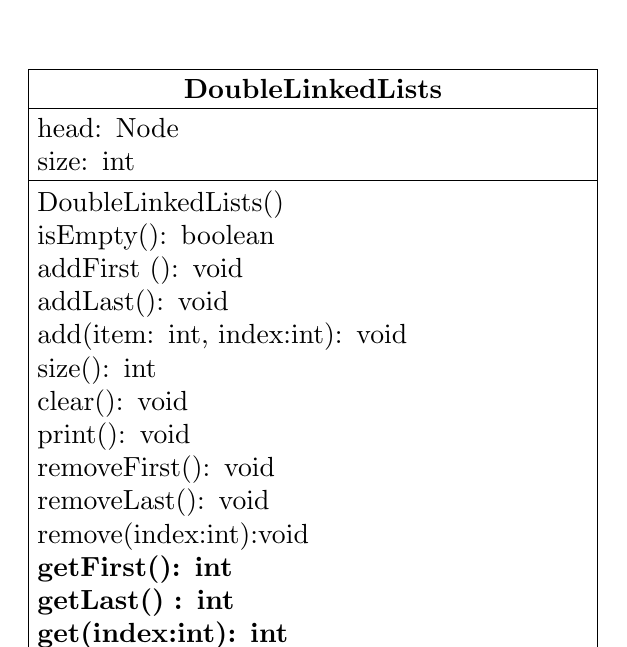
\begin{tikzpicture}
    \begin{class}[text width=7cm]{DoubleLinkedLists}{0,0}
        \attribute{head: Node}
        \attribute{size: int}
        \operation{DoubleLinkedLists()}
        \operation{isEmpty(): boolean}
        \operation{addFirst (): void}
        \operation{addLast(): void}
        \operation{add(item: int, index:int): void}
        \operation{size(): int}
        \operation{clear(): void}
        \operation{print(): void}
        \operation{removeFirst(): void}
        \operation{removeLast(): void}
        \operation{remove(index:int):void}
        \operation{ \textbf{getFirst(): int}}
        \operation{ \textbf{getLast() : int}}
        \operation{ \textbf{get(index:int): int}}
    \end{class}
\end{tikzpicture}
\mbox{}\\

\subsubsection{Steps}
\begin{enumerate}
    \item Create a method \textbf{getFirst()} in class \textbf{DoubleLinkedList} to retrieve the first data in the list
    \begin{minted}[autogobble,breaklines]{java}
        public int getFirst() throws Exception{
            if (isEmpty()) {
                throw new Exception("Linked list still empty");
            }
            return head.data;
        }
    \end{minted}
    \item Create a method \textbf{getLast()} in class \textbf{DoubleLinkedList} to retrieve the data in the list
    \begin{minted}[autogobble,breaklines]{java}
        public int getLast() throws Exception{
            if (isEmpty()) {
                throw new Exception("Linked list still empty");
            }
            Node temp = head;
            while (temp.next != null) {
                temp = temp.next;
            }
            return temp.data;
        }
    \end{minted}
    \item Create a method \textbf{get(int index)} in class \textbf{DoubleLinkedList} to retrieve the data in specified index of the list
    \begin{minted}[autogobble,breaklines]{java}
        public int get(int index) throws Exception{
            if (isEmpty()) {
                throw new Exception("Linked list still empty");
            }
            Node temp = head;
            for (int i = 0; i < index; i++) {
                temp = temp.next;
            }
            return temp.data;
        }
    \end{minted}
    \item In the main class, add the program code as follows and see the result
    \begin{minted}[autogobble,breaklines]{java}
        dll.print();
        System.out.println("Size: " + dll.size);
        System.out.println("================================================");
        dll.addFirst(3);
        dll.addLast(4);
        dll.addFirst(7);
        dll.print();
        System.out.println("Size: " + dll.size);
        System.out.println("================================================");

        dll.add(40,1);
        dll.print();

        System.out.println("Size: " + dll.size);
        System.out.println("================================================");
        System.out.println("Data in the head of the linked list is : " + dll.getFirst());
        System.out.println("Data in the tail of the linked list is : " + dll.getLast());
        System.out.println("Data in the 1st index of the linked list is : " + dll.get(1));
    \end{minted}
\end{enumerate}

\subsubsection{Result}
Compile the program and see if the result matches with following image
\begin{minted}[autogobble,breaklines,linenos]{text}
    PS D:\Kuliah\Smt 2\Algoritma dan Struktur Data\Praktikum\Week 12\Double Linked Lists>  d:; cd 'd:\Kuliah\Smt 2\Algoritma dan Struktur Data\Praktikum\Week 12\Double Linked Lists'; & 'C:\Program Files\Java\jdk-18.0.2.1\bin\java.exe' '-XX:+ShowCodeDetailsInExceptionMessages' '-cp' 'D:\Kuliah\Smt 2\Algoritma dan Struktur Data\Praktikum\Week 12\Double Linked Lists\bin' 'LabActivities.DoubleLinkedListMain' 
    Linked list is empty
    Size: 0
    ================================================
    7       3       4
    successfully added
    Size: 3
    ================================================
    7       40      3       4
    successfully added
    Size: 4
    ================================================
    Data in the head of the linked list is : 7
    Data in the tail of the linked list is : 4
    Data in the 1st index of the linked list is : 40
\end{minted}

\subsubsection{Questions}
\begin{enumerate}
    \item What is the function of method \textbf{size()} in \textbf{DoubleLinkedList} class ?
    \mbox{}\\
    \texttt{Answer: }
    \mbox{}\\
    return the size/length of the linked list
    \item How do we set the index in double linked list so that it starts from 1st index instead of 0th index?
    \mbox{}\\
    \texttt{Answer: }
    \mbox{}\\
    set the linked list size starting value to 1
    \item Please explain the difference between method \textbf{Add()} in double linked list and single linked list !
    \mbox{}\\
    \texttt{Answer: }
    \mbox{}\\
    the SLL only need to readjust next and tail while DLL need to change head, next, prev, and next, prev of prev, and next.  
    \item What’s the logic difference of these 2 following codes?
    \begin{enumerate}[label=(\alph*)]
        \item -
        \begin{minted}[autogobble,breaklines]{java}
            public boolean isEmpty() {
                if (size == 0) {
                    return true;
                } else {
                    return false;
                }
            }
        \end{minted}
        \item -
        \begin{minted}[autogobble,breaklines]{java}
            public boolean isEmpty() {
                return head == null;
            }
        \end{minted}
    \end{enumerate}
    \mbox{}\\
    \texttt{Answer: }
    \mbox{}\\
    the former check the size which in any case can be set at any size, while the later check the head of the linked list being sure it has the value of null. the later having better assurance over the former because if head is null its guarantee that the linked list is empty;
\end{enumerate}

\subsection{Assignment}
\begin{enumerate} 
    \item Create a program with double linked list implementation that allows user to choose a menu as following image! The searching uses sequential search approach and the program should be able to sort the data in descending order. You may any choose sorting approach you prefer (bubble sort, selection sort, insertion sort, or merge sort)
    \hbox{}\\\textbf{Adding a data}
    \hbox{}\\\textbf{Add data in specified index and display the result}
    \hbox{}\\\textbf{Search Data}
    \hbox{}\\\textbf{Sorting Data}
    
    \texttt{Node.java}
    \begin{minted}[autogobble,breaklines]{java}
        package Assignment;

        public class Node {
            int data;
            Node prev, next;

            public Node(Node prev, int data, Node next) {
                this.data = data;
                this.prev = prev;
                this.next = next;
            }
        }
    \end{minted}

    \texttt{DoubleLinkedList.java}
    \begin{minted}[autogobble,breaklines]{java}
        package Assignment;

        public class DoubleLinkedList {
            Node head;
            int size;

            public DoubleLinkedList() {
                head = null;
                size = 0;
            }

            public boolean isEmpty() {
                return head == null;
            }

            public void addFirst(int item) {
                if (isEmpty()) {
                    head = new Node(null, item, null);
                } else {
                    Node newNode = new Node(null, item, head);
                    head.prev = newNode;
                    head = newNode;
                }
                size++;
            }

            public void addLast(int item) {
                if (isEmpty()) {
                    addFirst(item);
                } else {
                    Node current = head;
                    while (current.next != null) {
                        current = current.next;
                    }
                    Node newNode = new Node(current, item, null);
                    current.next = newNode;
                    size++;
                }
            }

            public void add(int item, int index) throws Exception {
                if (isEmpty()) {
                    addFirst(item);
                } else if (index < 0 || index > size) {
                    throw new Exception("Index out of bound");
                } else {
                    Node current = head;
                    int i = 0;
                    while (i < index) {
                        current = current.next;
                        i++;
                    }
                    if (current.next == null) {
                        Node newNode = new Node(null, item, current);
                        current.prev = newNode;
                        head = newNode;
                    } else {
                        Node newNode = new Node(current.prev, item, current);
                        newNode.prev = current.prev;
                        newNode.next = current;
                        current.prev.next = newNode;
                        current.prev = newNode;
                    }
                }
                size++;
            }

            public int size() {
                return size;
            }

            public void clear() {
                head = null;
                size = 0;
            }

            public void print() {
                if (!isEmpty()) {
                    Node temp = head;
                    while (temp != null) {
                        System.out.print(temp.data + "\n");
                        temp = temp.next;
                    }
                    System.out.println("\n successfully added");
                } else {
                    System.out.println("Linked list is empty");
                }
            }

            public void removeFirst() throws Exception {
                if (isEmpty()) {
                    throw new Exception("Linked list is still empty, cannot remove data");
                } else if (size == 1) {
                    removeLast();
                } else {
                    head = head.next;
                    head.prev = null;
                    size--;
                }
            }

            public void removeLast() throws Exception {
                if (isEmpty()) {
                    throw new Exception("Linked list is still empty, cannot remove data");
                } else if (head.next == null) {
                    head = null;
                    size--;
                    return;
                } 
                Node current = head;
                while (current.next.next != null) {
                    current = current.next;
                }
                current.next = null;
                size--;
            }

            public void remove(int index) throws Exception {
                if (isEmpty() || index >= size) {
                    throw new Exception("Index value is out of bound");
                } else if (size == 0) {
                    removeFirst();
                } else {
                    Node current = head;
                    int i = 0;
                    while (i < index) {
                        current = current.next;
                        i++;
                    }
                    if (current.next == null) {
                        current.prev.next = null;
                    } else if (current.prev == null) {
                        current = current.next;
                        current.prev = null;
                        head = current;
                    } else {
                        current.prev.next = current.next;
                        current.next.prev = current.prev;
                    }
                    size--;
                }
            }

            public int getFirst() throws Exception {
                if (isEmpty()) {
                    throw new Exception("Linked list still empty");
                }
                return head.data;
            }

            public int getLast() throws Exception {
                if (isEmpty()) {
                    throw new Exception("Linked list still empty");
                }
                Node temp = head;
                while (temp.next != null) {
                    temp = temp.next;
                }
                return temp.data;
            }

            public int get(int index) throws Exception {
                if (isEmpty()) {
                    throw new Exception("Linked list still empty");
                }
                Node temp = head;
                for (int i = 0; i < index; i++) {
                    temp = temp.next;
                }
                return temp.data;
            }

            public int search(int key) throws Exception {
                Node temp = head;
                int i = 0;
                while (i < size) {
                    if (temp.data == key) {
                        return i;
                    }
                    i++;
                    temp = temp.next;
                }
                throw new Exception("Key value doesn't exist");
            }

            public void sort() throws Exception {
                if (head == null || head.next == null) {
                    return;
                }
                boolean swapped;
                Node current;
                Node last = null;
                do {
                    swapped = false;
                    current = head;
                    while (current.next != last) {
                        if (current.data > current.next.data) {
                            int temp = current.data;
                            current.data = current.next.data;
                            current.next.data = temp;
                            swapped = true;
                        }
                        current = current.next;
                    }
                    last = current;
                } while (swapped);
            }
        }

    \end{minted}

    \texttt{DoubleLinkedListMain.java}
    \begin{minted}[autogobble,breaklines]{java}
        package Assignment;

        import java.util.Scanner;

        public class DoubleLinkedListMain {
            public static void displayMenu() {
                System.out.println("=========================================");
                System.out.println("Data manipulation with Double Linked List");
                System.out.println("=========================================");
                System.out.println("1. Add First");
                System.out.println("2. Add Tail");
                System.out.println("3. Add Data in the nth index");
                System.out.println("4. Remove First");
                System.out.println("5. Remove Tail");
                System.out.println("6. Remove Data in the nth index");
                System.out.println("7. Print");
                System.out.println("8. Search Data");
                System.out.println("9. Sort Data");
                System.out.println("10. Exit");
                System.out.println("=========================================");
            }

            public static void main(String[] args) throws Exception {
                Scanner sc = new Scanner(System.in);
                DoubleLinkedList dll = new DoubleLinkedList();
                
                boolean exit = false;
                while (!exit) {
                    int option;
                    displayMenu();
                    option = sc.nextInt();
                    int dataAdd;
                    int posAdd;
                    int posDel;
                    int search;

                    switch (option) {
                        case 1:
                            System.out.println("Insert data in head position");
                            dataAdd = sc.nextInt();
                            dll.addFirst(dataAdd);
                            break;
                        case 2:
                            System.out.println("Insert data in last position");
                            dataAdd = sc.nextInt();
                            dll.addLast(dataAdd);
                            break;
                        case 3:
                            System.out.println("Insert Data");
                            System.out.print("Data node: ");
                            dataAdd = sc.nextInt();
                            System.out.print("In index: ");
                            posAdd = sc.nextInt();
                            dll.add(dataAdd, posAdd);
                            break;
                        case 4:
                            System.out.println("First Data deleted");
                            System.out.println(dll.getFirst());
                            dll.removeFirst();
                            break;
                        case 5:
                            System.out.println("Last Data deleted");
                            System.out.println(dll.getLast());
                            dll.removeLast();
                            break;
                        case 6:
                            System.out.println("Remove Data");
                            System.out.println("In index: ");
                            posDel = sc.nextInt();
                            System.out.println("Data " + posDel + " deleted");
                            System.out.println(dll.get(posDel));
                            dll.remove(posDel);
                            break;
                        case 7:
                            System.out.println("Print Data :");
                            dll.print();
                            break;
                        case 8:
                            System.out.print("Search Data :");
                            search = sc.nextInt();
                            System.out.printf("Data %d is in index-%d\n", search, dll.search(search));
                            break;
                        case 9:
                            dll.sort();
                            break;
                        case 10:
                            exit = true;
                            break;
                    }
                }
                
                sc.close();
            }
        }

    \end{minted}

    \begin{minted}[autogobble,breaklines,linenos]{text}
        PS D:\Kuliah\Smt 2\Algoritma dan Struktur Data\Praktikum\Week 12\Double Linked Lists>  d:; cd 'd:\Kuliah\Smt 2\Algoritma dan Struktur Data\Praktikum\Week 12\Double Linked Lists'; & 'C:\Program Files\Java\jdk-18.0.2.1\bin\java.exe' '-XX:+ShowCodeDetailsInExceptionMessages' '-cp' 'D:\Kuliah\Smt 2\Algoritma dan Struktur Data\Praktikum\Week 12\Double Linked Lists\bin' 'Assignment.DoubleLinkedListMain' 
        =========================================
        Data manipulation with Double Linked List
        =========================================
        1. Add First
        2. Add Tail
        3. Add Data in the nth index
        4. Remove First
        5. Remove Tail
        6. Remove Data in the nth index
        7. Print
        8. Search Data
        9. Sort Data
        10. Exit
        =========================================
        1
        Insert data in head position
        34
        =========================================
        Data manipulation with Double Linked List
        =========================================
        1. Add First
        2. Add Tail
        3. Add Data in the nth index
        4. Remove First
        5. Remove Tail
        6. Remove Data in the nth index
        7. Print
        8. Search Data
        9. Sort Data
        10. Exit
        =========================================
        2
        Insert data in last position
        10
        =========================================
        Data manipulation with Double Linked List
        =========================================
        1. Add First
        2. Add Tail
        3. Add Data in the nth index
        4. Remove First
        5. Remove Tail
        6. Remove Data in the nth index
        7. Print
        8. Search Data
        9. Sort Data
        10. Exit
        =========================================
        3
        Insert Data
        Data node: 66
        In index: 1
        =========================================
        Data manipulation with Double Linked List
        =========================================
        1. Add First
        2. Add Tail
        3. Add Data in the nth index
        4. Remove First
        5. Remove Tail
        6. Remove Data in the nth index
        7. Print
        8. Search Data
        9. Sort Data
        10. Exit
        =========================================
        8
        Search Data :66
        Data 66 is in index-0
        =========================================
        Data manipulation with Double Linked List
        =========================================
        1. Add First
        2. Add Tail
        3. Add Data in the nth index
        4. Remove First
        5. Remove Tail
        6. Remove Data in the nth index
        7. Print
        8. Search Data
        9. Sort Data
        10. Exit
        =========================================
        9
        =========================================
        Data manipulation with Double Linked List
        =========================================
        1. Add First
        2. Add Tail
        3. Add Data in the nth index
        4. Remove First
        5. Remove Tail
        6. Remove Data in the nth index
        7. Print
        8. Search Data
        9. Sort Data
        10. Exit
        =========================================
        7
        Print Data :
        10
        66

        successfully added
        =========================================
        Data manipulation with Double Linked List
        =========================================
        1. Add First
        2. Add Tail
        3. Add Data in the nth index
        4. Remove First
        5. Remove Tail
        6. Remove Data in the nth index
        7. Print
        8. Search Data
        9. Sort Data
        10. Exit
        =========================================
        7  
        Print Data :
        10
        66

        successfully added
        =========================================
        Data manipulation with Double Linked List
        =========================================
        1. Add First
        2. Add Tail
        3. Add Data in the nth index
        4. Remove First
        5. Remove Tail
        6. Remove Data in the nth index
        7. Print
        8. Search Data
        9. Sort Data
        10. Exit
        =========================================
        10
        PS D:\Kuliah\Smt 2\Algoritma dan Struktur Data\Praktikum\Week 12\Double Linked Lists>
    \end{minted}
    \item We are required to create a program which Implement Stack using double linked list. The features are described in following illustrations:
    \hbox{}\\\textbf{Initial menu and add Data (push)}
    \begin{minted}[autogobble,breaklines,linenos]{text}
        PS D:\Kuliah\Smt 2\Algoritma dan Struktur Data\Praktikum\Week 12\Double Linked Lists>  & 'C:\Program Files\Java\jdk-18.0.2.1\bin\java.exe' '-XX:+ShowCodeDetailsInExceptionMessages' '-cp' 'D:\Kuliah\Smt 2\Algoritma dan Struktur Data\Praktikum\Week 12\Double Linked Lists\bin' 'Assignment2.Main'
        ****************
        Library Data Book
        ****************
        1. Add new book
        2. Get book from top
        3. Peek book title from top
        4. Info all books
        5. Exit
        ****************
        1
        ------------------------
        Insert new book title
        ------------------------
        How to cuan
    \end{minted}
    \textbf{Print All Data}
    \begin{minted}[autogobble,breaklines,linenos]{text}
        ****************
        Library Data Book
        ****************
        1. Add new book
        2. Get book from top
        3. Peek book title from top
        4. Info all books
        5. Exit
        ****************
        4
        ------------------------
        info all books
        ------------------------
        How to cuan
    \end{minted}
    \textbf{See the data on top of the stack}
    \begin{minted}[autogobble,breaklines,linenos]{text}
        ****************
        Library Data Book
        ****************
        1. Add new book
        2. Get book from top
        3. Peek book title from top
        4. Info all books
        5. Exit
        ****************
        3
        ------------------------
        Peek book title from top
        ------------------------
        How to cuan
    \end{minted}
    \textbf{Pop the data from the top of the stack}
    \begin{minted}[autogobble,breaklines,linenos]{text}
        ****************
        Library Data Book
        ****************
        1. Add new book
        2. Get book from top
        3. Peek book title from top
        4. Info all books
        5. Exit
        ****************
        2
        ------------------------
        Book on top has been removed
        ------------------------
        ****************
        Library Data Book
        ****************
        1. Add new book
        2. Get book from top
        3. Peek book title from top
        4. Info all books
        5. Exit
        ****************
        4
        ------------------------
        info all books
        ------------------------
        Linked list is empty
        ****************
        Library Data Book
        ****************
        1. Add new book
        2. Get book from top
        3. Peek book title from top
        4. Info all books
        5. Exit
        ****************
        5
    \end{minted}
    \texttt{Node.java}
    \begin{minted}[autogobble,breaklines]{java}
        package Assignment2;

        public class Node {
            String data;
            Node prev, next;

            public Node(Node prev, String data, Node next) {
                this.data = data;
                this.prev = prev;
                this.next = next;
            }
        }
    \end{minted}
    \texttt{DoubleLinkedList.java}
    \begin{minted}[autogobble,breaklines]{java}
        package Assignment2;

        public class DoubleLinkedList {
            Node head;
            int size;

            public DoubleLinkedList() {
                head = null;
                size = 0;
            }

            public boolean isEmpty() {
                return head == null;
            }

            public void addFirst(String item) {
                if (isEmpty()) {
                    head = new Node(null, item, null);
                } else {
                    Node newNode = new Node(null, item, head);
                    head.prev = newNode;
                    head = newNode;
                }
                size++;
            }

            public int size() {
                return size;
            }

            public void clear() {
                head = null;
                size = 0;
            }

            public void print() {
                if (!isEmpty()) {
                    Node temp = head;
                    while (temp != null) {
                        System.out.print(temp.data + "\n");
                        temp = temp.next;
                    }
                } else {
                    System.out.println("Linked list is empty");
                }
            }

            public void removeFirst() throws Exception {
                if (isEmpty()) {
                    throw new Exception("Linked list is still empty, cannot remove data");
                } else if (size == 1) {
                    removeLast();
                } else {
                    head = head.next;
                    head.prev = null;
                    size--;
                }
            }

            public void removeLast() throws Exception {
                if (isEmpty()) {
                    throw new Exception("Linked list is still empty, cannot remove data");
                } else if (head.next == null) {
                    head = null;
                    size--;
                    return;
                } 
                Node current = head;
                while (current.next.next != null) {
                    current = current.next;
                }
                current.next = null;
                size--;
            }

            public String getFirst() throws Exception {
                if (isEmpty()) {
                    throw new Exception("Linked list still empty");
                }
                return head.data;
            }
        }
    \end{minted}
    \texttt{Main.java}
    \begin{minted}[autogobble,breaklines]{java}
        package Assignment2;

        import java.util.Scanner;

        public class Main {
            static Scanner sc = new Scanner(System.in);
            static DoubleLinkedList dll = new DoubleLinkedList();
            public static void displayMenu() {
                System.out.println("****************");
                System.out.println("Library Data Book");
                System.out.println("****************");
                System.out.println("1. Add new book");
                System.out.println("2. Get book from top");
                System.out.println("3. Peek book title from top");
                System.out.println("4. Info all books");
                System.out.println("5. Exit");
                System.out.println("****************");
            }
            
            public static void add() throws Exception {
                System.out.println("------------------------");
                System.out.println("Insert new book title");
                System.out.println("------------------------");
                sc.nextLine();
                String data = sc.nextLine();
                dll.addFirst(data);
                pivot();
            }
            
            public static void pop() throws Exception {
                System.out.println("------------------------");
                System.out.println("Book on top has been removed");
                System.out.println("------------------------");
                dll.removeFirst();
                pivot();
            }

            public static void peek() throws Exception {
                System.out.println("------------------------");
                System.out.println("Peek book title from top");
                System.out.println("------------------------");
                System.out.println(dll.getFirst());
                pivot();
            }

            public static void print() throws Exception {
                System.out.println("------------------------");
                System.out.println("info all books");
                System.out.println("------------------------");
                dll.print();
                pivot();
            }

            public static void exit() {
                sc.close();
            }
            
            public static void pivot() throws Exception {
                displayMenu();
                int option = sc.nextInt();
                switch (option) {
                    case 1 -> add();
                    case 2 -> pop();
                    case 3 -> peek();
                    case 4 -> print();
                    case 5 -> exit();
                }
            }
            
            public static void main(String[] args) throws Exception {
                pivot();
                sc.close();
            }
        }

    \end{minted}
    \item Create a program that helps vaccination process by having a queue algorithm alongside with double linked list as follows \textbf{(the amount left of queue length in menu print(3) and recent vaccinated person in menu Remove data (2) should be displayed)}
    \hbox{}\\\textbf{Initial menu and adding a data}
    \begin{minted}[autogobble,breaklines,linenos]{text}
        PS D:\Kuliah\Smt 2\Algoritma dan Struktur Data\Praktikum\Week 12\Double Linked Lists>  d:; cd 'd:\Kuliah\Smt 2\Algoritma dan Struktur Data\Praktikum\Week 12\Double Linked Lists'; & 'C:\Program Files\Java\jdk-18.0.2.1\bin\java.exe' '-XX:+ShowCodeDetailsInExceptionMessages' '-cp' 'D:\Kuliah\Smt 2\Algoritma dan Struktur Data\Praktikum\Week 12\Double Linked Lists\bin' 'Assignment3.Main' 
        ++++++++++++++++++++++++++
        Extravaganza Vaccine Queue
        ++++++++++++++++++++++++++
        1. Add vaccine queue
        2. Remove vaccine queue
        3. Display vaccine queue
        4. Exit
        ++++++++++++++++++++++++++
        1
        Add vaccine queue
        Queue number : 123
        Name : joko
    \end{minted}
    \textbf{Print data (notice the highlighted red in the result)}
    \begin{minted}[autogobble,breaklines,linenos]{text}
        ++++++++++++++++++++++++++
        Extravaganza Vaccine Queue
        ++++++++++++++++++++++++++
        1. Add vaccine queue
        2. Remove vaccine queue
        3. Display vaccine queue
        4. Exit
        ++++++++++++++++++++++++++
        3
        current vaccine queue : 
        |No.   |Name    |
        |123   |joko    |
        Queue left : 1
    \end{minted}
    \textbf{Remove Data (the highlighted red must displayed in the console too)}
    \begin{minted}[autogobble,breaklines,linenos]{text}
        ++++++++++++++++++++++++++
        Extravaganza Vaccine Queue
        ++++++++++++++++++++++++++
        1. Add vaccine queue
        2. Remove vaccine queue
        3. Display vaccine queue
        4. Exit
        ++++++++++++++++++++++++++
        2
        joko has been vaccinated !
        ++++++++++++++++++++++++++
        Extravaganza Vaccine Queue
        ++++++++++++++++++++++++++
        1. Add vaccine queue
        2. Remove vaccine queue
        3. Display vaccine queue
        4. Exit
        ++++++++++++++++++++++++++
        4
    \end{minted}
    \texttt{Person.java}
    \begin{minted}[autogobble,breaklines]{java}
        package Assignment3;

        public class Person {
            String name;
            int queue;

            public Person(String name, int queue) {
                this.name = name;
                this.queue = queue;
            }
        }
    \end{minted}
    \texttt{Node.java}
    \begin{minted}[autogobble,breaklines]{java}
        package Assignment3;

        public class Node {
            Person data;
            Node prev, next;

            public Node(Node prev, Person data, Node next) {
                this.data = data;
                this.prev = prev;
                this.next = next;
            }
        }
    \end{minted}
    \texttt{DoubleLinkedList.java}
    \begin{minted}[autogobble,breaklines]{java}
        package Assignment3;

        public class DoubleLinkedList {
            Node head;
            int size;

            public DoubleLinkedList() {
                head = null;
                size = 0;
            }

            public boolean isEmpty() {
                return head == null;
            }

            public void addFirst(Person item) {
                if (isEmpty()) {
                    head = new Node(null, item, null);
                } else {
                    Node newNode = new Node(null, item, head);
                    head.prev = newNode;
                    head = newNode;
                }
                size++;
            }

            public void addLast(Person item) {
                if (isEmpty()) {
                    addFirst(item);
                } else {
                    Node current = head;
                    while (current.next != null) {
                        current = current.next;
                    }
                    Node newNode = new Node(current, item, null);
                    current.next = newNode;
                    size++;
                }
            }

            public int size() {
                return size;
            }

            public void clear() {
                head = null;
                size = 0;
            }

            public void print() {
                if (!isEmpty()) {
                    Node temp = head;
                    int count = 0;
                    System.out.println("|No.   |Name    |");
                    while (temp != null) {
                        System.out.printf("|%-6d|%-8s|\n", temp.data.queue, temp.data.name);
                        count++;
                        temp = temp.next;
                    }
                    System.out.printf("Queue left : %d\n", count);
                } else {
                    System.out.println("Linked list is empty");
                }
            }

            public void removeFirst() throws Exception {
                if (isEmpty()) {
                    throw new Exception("Linked list is still empty, cannot remove data");
                } else if (size == 1) {
                    removeLast();
                } else {
                    head = head.next;
                    head.prev = null;
                    size--;
                }
            }

            public void removeLast() throws Exception {
                if (isEmpty()) {
                    throw new Exception("Linked list is still empty, cannot remove data");
                } else if (head.next == null) {
                    head = null;
                    size--;
                    return;
                } 
                Node current = head;
                while (current.next.next != null) {
                    current = current.next;
                }
                current.next = null;
                size--;
            }

            public String getFirst() throws Exception {
                if (isEmpty()) {
                    throw new Exception("Linked list still empty");
                }
                return head.data.name;
            }
        }

    \end{minted}
    \texttt{Main.java}
    \begin{minted}[autogobble,breaklines]{java}
        package Assignment3;

        import java.util.Scanner;

        public class Main {
            static Scanner sc = new Scanner(System.in);
            static DoubleLinkedList dll = new DoubleLinkedList();
            public static void displayMenu() {
                System.out.println("++++++++++++++++++++++++++");
                System.out.println("Extravaganza Vaccine Queue");
                System.out.println("++++++++++++++++++++++++++");
                System.out.println("1. Add vaccine queue");
                System.out.println("2. Remove vaccine queue");
                System.out.println("3. Display vaccine queue");
                System.out.println("4. Exit");
                System.out.println("++++++++++++++++++++++++++");
            }
            
            public static void add() throws Exception {
                System.out.println("Add vaccine queue");
                System.out.print("Queue number : ");
                int queueNumber = sc.nextInt();
                System.out.print("Name : ");
                sc.nextLine();
                String name = sc.nextLine();
                Person data = new Person(name, queueNumber);
                dll.addFirst(data);
                pivot();
            }
            
            public static void pop() throws Exception {
                System.out.printf("%s has been vaccinated !\n", dll.getFirst());
                dll.removeLast();
                pivot();
            }

            public static void print() throws Exception {
                System.out.println("current vaccine queue : ");
                dll.print();
                pivot();
            }

            public static void exit() {
                sc.close();
            }
            
            public static void pivot() throws Exception {
                displayMenu();
                int option = sc.nextInt();
                switch (option) {
                    case 1 -> add();
                    case 2 -> pop();
                    case 3 -> print();
                    case 4 -> exit();
                }
            }
            
            public static void main(String[] args) throws Exception {
                pivot();
                sc.close();
            }
        }
    \end{minted}
    \item Create a program implementation that list students score. Each student’s data consist of their nim, name, and gpa. The program should implement double linked list and should be able to search based on NIM and sort the GPA in descending order. \textbf{Students class must be implemented in this program}
    \hbox{}\\\textbf{Initial menu and adding data}
    \begin{minted}[autogobble,breaklines,linenos]{text}
        PS D:\Kuliah\Smt 2\Algoritma dan Struktur Data\Praktikum\Week 12\Double Linked Lists>  d:; cd 'd:\Kuliah\Smt 2\Algoritma dan Struktur Data\Praktikum\Week 12\Double Linked Lists'; & 'C:\Program Files\Java\jdk-18.0.2.1\bin\java.exe' '-XX:+ShowCodeDetailsInExceptionMessages' '-cp' 'D:\Kuliah\Smt 2\Algoritma dan Struktur Data\Praktikum\Week 12\Double Linked Lists\bin' 'Assignment4.Main' 
        =============================== 
        Student Data Management System  
        =============================== 
        1. Add data from head
        2. Add data from Tail
        3. Add data in specific index   
        4. Remove data from head        
        5. Remove data from Tail        
        6. Remove data in specific index
        7. Print
        8. Search by NIM
        9. Sort by GPA - Desc
        10. Exit
        =============================== 
        1
        Insert NIM in head position
        NIM  : 123
        Name : Anang
        GPA  : 2.77
        =============================== 
        Student Data Management System  
        =============================== 
        1. Add data from head
        2. Add data from Tail
        3. Add data in specific index   
        4. Remove data from head
        5. Remove data from Tail
        6. Remove data in specific index
        7. Print
        8. Search by NIM
        9. Sort by GPA - Desc
        10. Exit
        ===============================
        2
        Insert NIM in tail position
        NIM  : 233
        Name : Suparjo
        GPA  : 3.67
        =============================== 
        Student Data Management System
        ===============================
        1. Add data from head
        2. Add data from Tail
        3. Add data in specific index
        4. Remove data from head
        5. Remove data from Tail
        6. Remove data in specific index
        7. Print
        8. Search by NIM
        9. Sort by GPA - Desc
        10. Exit
        ===============================
        3
        Insert student's data node
        NIM  : 743
        Name : Freddy
        GPA  : 2.90
        In index : 2
    \end{minted}
    \textbf{Printing data}
    \begin{minted}[autogobble,breaklines,linenos]{text}
        =============================== 
        Student Data Management System
        ===============================
        1. Add data from head
        2. Add data from Tail
        3. Add data in specific index
        4. Remove data from head
        5. Remove data from Tail
        6. Remove data in specific index
        7. Print
        8. Search by NIM
        9. Sort by GPA - Desc
        10. Exit
        ===============================
        7
        ================================
        NIM  : 123
        Name : Anang
        GPA  : 2.77
        ================================
        NIM  : 233
        Name : Suparjo
        GPA  : 3.67
        ================================
        NIM  : 743
        Name : Freddy
        GPA  : 2.90

        All data printed successfully
    \end{minted}
    \textbf{Searching data}
    \begin{minted}[autogobble,breaklines,linenos]{text}
        ===============================
        Student Data Management System
        ===============================
        1. Add data from head
        2. Add data from Tail
        3. Add data in specific index
        4. Remove data from head
        5. Remove data from Tail
        6. Remove data in specific index
        7. Print
        8. Search by NIM
        9. Sort by GPA - Desc
        10. Exit
        ===============================
        8
        Insert NIM to be searched : 233
        Data 233 is in node - 1
        Identity :
        ================================
        NIM  : 233
        Name : Suparjo
        GPA  : 3.67
    \end{minted}
    \textbf{Sorting data}
    \begin{minted}[autogobble,breaklines,linenos]{text}
        ===============================
        Student Data Management System
        ===============================
        1. Add data from head
        2. Add data from Tail
        3. Add data in specific index
        4. Remove data from head
        5. Remove data from Tail
        6. Remove data in specific index
        7. Print
        8. Search by NIM
        9. Sort by GPA - Desc
        10. Exit
        ===============================
        9
        =============================== 
        Student Data Management System
        ===============================
        1. Add data from head
        2. Add data from Tail
        3. Add data in specific index
        4. Remove data from head
        5. Remove data from Tail
        6. Remove data in specific index
        7. Print
        8. Search by NIM
        9. Sort by GPA - Desc
        10. Exit
        ===============================
        7
        ================================
        NIM  : 233
        Name : Suparjo
        GPA  : 3.67
        ================================
        NIM  : 743
        Name : Freddy
        GPA  : 2.90
        ================================
        NIM  : 123
        Name : Anang
        GPA  : 2.77

        All data printed successfully
        ===============================
        Student Data Management System
        ===============================
        1. Add data from head
        2. Add data from Tail
        3. Add data in specific index
        4. Remove data from head
        5. Remove data from Tail
        6. Remove data in specific index
        7. Print
        8. Search by NIM
        9. Sort by GPA - Desc
        10. Exit
        ===============================
        10
    \end{minted}

    \texttt{Student.java}
    \begin{minted}[autogobble,breaklines]{java}
        package Assignment4;

        public class Student {
            String name;
            int nim;
            double gpa;

            public Student(String name, int NIM, double GPA) {
                this.name = name;
                this.nim = NIM;
                this.gpa = GPA;
            }

            public void print() {
                System.out.println("================================");
                System.out.printf("NIM  : %d\n", nim);
                System.out.printf("Name : %s\n", name);
                System.out.printf("GPA  : %.2f\n", gpa);
            }
        }
    \end{minted}
    \texttt{Node.java}
    \begin{minted}[autogobble,breaklines]{java}
        package Assignment4;

        public class Node {
            Student data;
            Node prev, next;

            public Node(Node prev, Student data, Node next) {
                this.data = data;
                this.prev = prev;
                this.next = next;
            }
        }
    \end{minted}
    \texttt{DoubleLinkedList.java}
    \begin{minted}[autogobble,breaklines]{java}
        package Assignment4;

        public class DoubleLinkedList {
            Node head;
            int size;

            public DoubleLinkedList() {
                head = null;
                size = 0;
            }

            public boolean isEmpty() {
                return head == null;
            }

            public void addFirst(Student item) {
                if (isEmpty()) {
                    head = new Node(null, item, null);
                } else {
                    Node newNode = new Node(null, item, head);
                    head.prev = newNode;
                    head = newNode;
                }
                size++;
            }

            public void addLast(Student item) {
                if (isEmpty()) {
                    addFirst(item);
                } else {
                    Node current = head;
                    while (current.next != null) {
                        current = current.next;
                    }
                    Node newNode = new Node(current, item, null);
                    current.next = newNode;
                    size++;
                }
            }

            public void add(Student item, int index) throws Exception {
                if (isEmpty()) {
                    addFirst(item);
                } else if (index < 0 || index > size) {
                    throw new Exception("Index out of bound");
                } else if (index == size) {
                    addLast(item);
                } else {
                    Node current = head;
                    int i = 0;
                    while (i < index) {
                        current = current.next;
                        i++;
                    }
                    if (current.next == null) {
                        Node newNode = new Node(null, item, current);
                        current.prev = newNode;
                        head = newNode;
                    } else {
                        Node newNode = new Node(current.prev, item, current);
                        newNode.prev = current.prev;
                        newNode.next = current;
                        current.prev.next = newNode;
                        current.prev = newNode;
                    }
                }
                size++;
            }

            public int size() {
                return size;
            }

            public void clear() {
                head = null;
                size = 0;
            }

            public void print() {
                if (!isEmpty()) {
                    Node temp = head;
                    while (temp != null) {
                        temp.data.print();
                        temp = temp.next;
                    }
                    System.out.println("\nAll data printed successfully");
                } else {
                    System.out.println("Linked list is empty");
                }
            }

            public void removeFirst() throws Exception {
                if (isEmpty()) {
                    throw new Exception("Linked list is still empty, cannot remove data");
                } else if (size == 1) {
                    removeLast();
                } else {
                    head = head.next;
                    head.prev = null;
                    size--;
                }
            }

            public void removeLast() throws Exception {
                if (isEmpty()) {
                    throw new Exception("Linked list is still empty, cannot remove data");
                } else if (head.next == null) {
                    head = null;
                    size--;
                    return;
                } 
                Node current = head;
                while (current.next.next != null) {
                    current = current.next;
                }
                current.next = null;
                size--;
            }

            public void remove(int index) throws Exception {
                if (isEmpty() || index >= size) {
                    throw new Exception("Index value is out of bound");
                } else if (size == 0) {
                    removeFirst();
                } else {
                    Node current = head;
                    int i = 0;
                    while (i < index) {
                        current = current.next;
                        i++;
                    }
                    if (current.next == null) {
                        current.prev.next = null;
                    } else if (current.prev == null) {
                        current = current.next;
                        current.prev = null;
                        head = current;
                    } else {
                        current.prev.next = current.next;
                        current.next.prev = current.prev;
                    }
                    size--;
                }
            }

            public Student getFirst() throws Exception {
                if (isEmpty()) {
                    throw new Exception("Linked list still empty");
                }
                return head.data;
            }

            public Student getLast() throws Exception {
                if (isEmpty()) {
                    throw new Exception("Linked list still empty");
                }
                Node temp = head;
                while (temp.next != null) {
                    temp = temp.next;
                }
                return temp.data;
            }

            public Student get(int index) throws Exception {
                if (isEmpty()) {
                    throw new Exception("Linked list still empty");
                }
                Node temp = head;
                for (int i = 0; i < index; i++) {
                    temp = temp.next;
                }
                return temp.data;
            }
            public int search(int key) throws Exception {
                Node temp = head;
                int i = 0;
                while (i < size) {
                    if (temp.data.nim == key) {
                        return i;
                    }
                    i++;
                    temp = temp.next;
                }
                throw new Exception("Key value doesn't exist");
            }

            public void sort() throws Exception {
                if (head == null || head.next == null) {
                    return;
                }
                boolean swapped;
                Node current;
                Node last = null;
                do {
                    swapped = false;
                    current = head;
                    while (current.next != last) {
                        if (current.data.gpa < current.next.data.gpa) {
                            Student temp = current.data;
                            current.data = current.next.data;
                            current.next.data = temp;
                            swapped = true;
                        }
                        current = current.next;
                    }
                    last = current;
                } while (swapped);
            }
        }
    \end{minted}
    \texttt{Main.java}
    \begin{minted}[autogobble,breaklines]{java}
        package Assignment4;

        import java.util.Scanner;

        public class Main {
            static Scanner sc = new Scanner(System.in);
            static DoubleLinkedList dll = new DoubleLinkedList();

            public static void displayMenu() {
                System.out.println("=============================== ");
                System.out.println("Student Data Management System  ");
                System.out.println("=============================== ");
                System.out.println("1. Add data from head           ");
                System.out.println("2. Add data from Tail           ");
                System.out.println("3. Add data in specific index   ");
                System.out.println("4. Remove data from head        ");
                System.out.println("5. Remove data from Tail        ");
                System.out.println("6. Remove data in specific index");
                System.out.println("7. Print                        ");
                System.out.println("8. Search by NIM                ");
                System.out.println("9. Sort by GPA - Desc           ");
                System.out.println("10. Exit                        ");
                System.out.println("=============================== ");
            }

            public static Student newStudent() {
                System.out.print("NIM  : ");
                int NIM = sc.nextInt();
                System.out.print("Name : ");
                sc.nextLine();
                String name = sc.nextLine();
                System.out.print("GPA  : ");
                double GPA = sc.nextDouble();
                Student data = new Student(name, NIM, GPA);
                return data;
            }

            public static void addFirst() throws Exception {
                System.out.println("Insert NIM in head position");
                Student data = newStudent();
                dll.addFirst(data);
                pivot();
            }

            public static void addLast() throws Exception {
                System.out.println("Insert NIM in tail position");
                Student data = newStudent();
                dll.addLast(data);
                pivot();
            }

            public static void add() throws Exception {
                System.out.println("Insert student's data node");
                Student data = newStudent();
                System.out.print("In index : ");
                int index = sc.nextInt();
                dll.add(data, index);
                pivot();
            }

            public static void removeFirst() throws Exception {
                System.out.println("Insert NIM in head position");
                dll.removeFirst();
                pivot();
            }

            public static void removeLast() throws Exception {
                System.out.println("Insert NIM in tail position");
                dll.removeLast();
                pivot();
            }
            public static void remove() throws Exception {
                System.out.println("Insert student's data node");
                System.out.print("In index : ");
                int index = sc.nextInt();
                dll.remove(index);
                pivot();
            }

            public static void print() throws Exception {
                dll.print();
                pivot();
            }

            public static void search() throws Exception {
                System.out.print("Insert NIM to be searched : ");
                int key = sc.nextInt();
                System.out.printf("Data %d is in node - %d\n", key, dll.search(key));
                System.out.println("Identity : ");
                dll.get(dll.search(key)).print();
                pivot();
            }

            public static void sort() throws Exception {
                dll.sort();
                pivot();
            }

            public static void exit() {
                sc.close();
            }

            public static void pivot() throws Exception {
                displayMenu();
                int option = sc.nextInt();
                switch (option) {
                    case 1  -> addFirst();
                    case 2  -> addLast();
                    case 3  -> add();
                    case 4  -> removeFirst();
                    case 5  -> removeLast();
                    case 6  -> remove();
                    case 7  -> print();
                    case 8  -> search();
                    case 9  -> sort();
                    case 10 -> exit();
                }
            }

            public static void main(String[] args) throws Exception {
                pivot();
                sc.close();
            }
        }
    \end{minted}
\end{enumerate}

\end{document}